The evaluation addresses five research questions, each answered by the sections
noted below.

\emph{(RQ1) End-to-end utility.} Does GPB improve the operating point across
dataset--backbone settings, and which design factor carries the gain? The main
results (Sec.~\ref{sec:main-results}) report the former, and the
paired factor-wise attribution ladder (Sec.~\ref{sec:ablation}) isolates the latter.

\emph{(RQ2) Comparator floor.} Does the trained posterior attain the theoretically
predicted ambiguity floor and never leave the explicit comparator's reachable set?
The controlled label-noise study varies a known floor from zero to $11.2$ nats and
checks the comparator gate (Sec.~\ref{sec:controlled-validation}).

\emph{(RQ3) Geometry transfer and certification.} How much of the declared prior
geometry reaches the learned posterior, and does the separation guarantee survive
the measured mismatch? The posterior alignment and separation study measures the transfer, and the
geometry-transfer study verifies the posterior-side structure (Secs.~\ref{sec:direct-mismatch}
and \ref{sec:mechanism}).

\emph{(RQ4) Compression behavior.} What do the methods compress and discard along
the $\beta$ sweep, and how does the anchor scale trade accuracy against
compression? The compression curves and the information-plane estimates read both
(Secs.~\ref{sec:sweep} and \ref{sec:info-plane}).

\emph{(RQ5) Robustness.} Does the compressed geometric operating point reduce
targeted adversarial success without giving up clean accuracy? The white-box PGD
study answers it (Sec.~\ref{sec:robustness}).

\subsection{Experimental setup}
\label{sec:setup}
We evaluate twelve dataset--backbone settings over nine public datasets:
MNIST, ImageNet-100, Cora, IMDb, AG News, California Housing, STS-B,
ZINC-12k, and AgeDB, covering MLP, CNN, GCN, and RNN backbones. All
methods use the same data splits ($60/20/20$ train/validation/test for
most datasets), backbone, Adam training, early stopping,
validation-based selection, and ten seeds per configuration. The baselines are Base, VIB,
SVIB, NIB, CEB, supervised $\beta$-DVCCA, and the external non-IB
baselines NCBD and AdaCap; GPB is OPB on classification rows and EPB on
regression rows. The main comparison is single-dimensional in tuned
hyperparameters: the plain backbone has no method-specific
hyperparameters, every $\beta$-weighted method is swept over the same
six-point $\beta$ grid, and NCBD and AdaCap use six-value grids of their
own. GPB's anchor scale $a$ (resp.\ isometric scale $\rho$) is a
trainable model parameter, shared across classes and clipped to
$[1,20]$ during training, so GPB receives no
larger tuning budget than the others. For each method and setting,
the configuration with the best mean validation metric is selected
(accuracy on classification settings, $R^2$ on regression settings). The
reported results are means with standard deviations over seeds, and
paired differences use $95\%$ bootstrap confidence intervals. The complete
experimental setup is in Appendix~\ref{app:setup-details}.

\subsection{Main results}
\label{sec:main-results}
% 主结果表：由 paper/make_table.py 从 tune_results/*.html 自动生成，请勿手改。
% 分类任务为测试 Acc（%）、回归任务为测试 R²；均为 5 次运行均值（不含标准差）。
% 每格取该模型在 β / anchor-scale 调参网格上的最优配置（tune_results 各表绿色高亮行），
% 每行（数据集）的最优指标加粗、次优（并列次优全部）加下划线；表尾两行统计各方法跨行的平均排名（越低越好）与最优/并列最优次数。
\begin{table*}[t]
\centering
\caption{Test accuracy (\%) on classification tasks and test $R^2$ on regression tasks (mean over 5 runs). Each entry reports the best configuration over the tuned $\beta$ (and anchor-scale) grid; the best entry per dataset is bolded.}
\label{tab:main_result}
\small
{
\setlength{\tabcolsep}{2pt}
\begin{tabular}{llcccccc|cc}
\hline
Dataset & Backbone & Base & VIB & SVIB & NIB & CEB & DVCCA & GPB & OPB-L \\
\hline
MNIST & MLP & 98.33 & 98.28 & 98.15 & 98.27 & \underline{98.43} & 98.24 & \textbf{98.54} & \underline{98.43} \\
MNIST & CNN & 99.13 & 99.28 & 99.23 & 99.22 & 99.30 & 99.29 & \textbf{99.32} & \underline{99.31} \\
ImageNet-100 & MLP & 83.12 & 82.84 & 83.02 & 82.35 & 82.77 & 82.99 & \textbf{84.40} & \underline{84.01} \\
ImageNet-100 & CNN & 83.40 & 82.94 & 83.11 & 82.91 & 82.97 & 83.21 & \textbf{86.08} & \underline{84.88} \\
Cora & GCN & 87.68 & 86.83 & 86.46 & 86.35 & 86.27 & 86.90 & \textbf{88.12} & \underline{87.86} \\
IMDb & RNN & 84.85 & 85.50 & 85.99 & 86.14 & 85.55 & 85.69 & \underline{86.84} & \textbf{86.99} \\
AG News & RNN & \textbf{92.94} & 92.72 & 92.86 & 92.91 & 92.83 & 92.78 & 92.87 & \underline{92.92} \\
\hline\hline
Cal. Housing & MLP & 0.7618 & \underline{0.7901} & 0.7897 & 0.7862 & 0.7894 & 0.7878 & 0.7895 & \textbf{0.7914} \\
STS-B & RNN & \textbf{0.2899} & 0.2719 & 0.2697 & 0.2417 & 0.2668 & 0.2713 & \underline{0.2762} & 0.2755 \\
ZINC & GCN & \textbf{0.6348} & 0.6339 & 0.6325 & 0.6178 & 0.6257 & 0.6294 & \underline{0.6344} & 0.6323 \\
AgeDB & MLP & 0.2180 & 0.3173 & \underline{0.3385} & 0.2710 & 0.3317 & 0.3180 & \textbf{0.3536} & 0.3320 \\
AgeDB & CNN & 0.3914 & 0.3342 & 0.3323 & 0.3337 & 0.3882 & 0.3205 & \textbf{0.4700} & \underline{0.4388} \\
\hline
\multicolumn{2}{l}{Mean rank (of 12)} & 4.25 & 5.25 & 5.00 & 6.50 & 5.46 & 5.50 & 1.75 & 2.29 \\
\multicolumn{2}{l}{Best or tied-best (of 12)} & 3 & 0 & 0 & 0 & 0 & 0 & 7 & 2 \\
\hline
\end{tabular}
}
\end{table*}

Table~\ref{tab:main_result} reports the best validation-selected configuration of
every baseline and GPB variant; the complete standard deviations and paired confidence
intervals are in Appendices~\ref{app:main-std} and \ref{app:main-ci};
per-method configuration details are in Appendix~\ref{app:setup-details}. The ranking summary is dominated by GPB: it has
the lowest mean rank ($1.58$ versus $4.08$ for the best plain
baseline) and is best or tied-best in $8/12$ settings. The gains are largest where the task has margin to
resolve them: on ImageNet-100 (CNN) GPB leads CEB by $3.11$ points and on Cora by
$1.85$, while the saturated settings are flat (MNIST CNN and AG News, where all
methods sit within $0.6$ points of the best) and the small-data regressions are
essentially tied with the best baselines (Housing within $0.0006$ $R^2$ of VIB; on
STS-B the plain backbone remains best). Among the external non-IB baselines, AdaCap is
competitive on regression (best on ZINC), while NCBD's mean rank ($5.43$) places it
behind the plain backbone on classification. Across modalities, the same construction
improves the operating point where improvement is available and costs nothing
elsewhere.

\subsection{Controlled label noise}
\label{sec:controlled-validation}
Theorem~\ref{prop:pgib-alignment}'s certificate assumes $\varepsilon$-optimality of
the fitted solution, which non-convex training does not guarantee; the controlled
experiment checks this premise and the certificate's tightness where the comparator
floor is analytically known. It isolates the comparator floor by making the
label-ambiguity term of the mismatch bound analytically known, and verifies three
claims: the noise-free case realizes the zero floor exactly, the measured mismatch
tracks the analytic floor at every noise level, and the fitted objective never
leaves the explicit comparator's reachable set. The construction uses $K=10$,
$X=e_C$, and symmetric
label noise $r_{\rm n}\in\{0,0.1,0.2,0.4\}$ with OPB $(a,\tau)=(6,1)$. The analytic
ambiguity floor (Appendix~\ref{app:noisy-alignment-sensitivity}) grows from $0$ to
$11.2$ nats as $r_{\rm n}$ runs over the noise grid. The explicit comparator takes
posterior mean $h_0(x)=a\sum_k\eta_k(x)q_k$ and covariance $\tau^2I$, where
$\eta_k(x)=P(Y=k\mid X=x)$; its KL equals $\delta_{\rm noise}(r_{\rm n})$ exactly (Proposition~\ref{prop:pgib-ambiguity-decomposition}), and its
anchor-energy risk is $C_{\rm comp}(r_{\rm n})$. The training protocol (population-weighted
objective, warm start, Monte Carlo risk estimation) is in
Appendix~\ref{app:noisy-alignment-sensitivity}. Whenever the
fitted objective satisfies $\widehat L\le L_{\rm comp}=C_{\rm comp}+\beta\delta_{\rm noise}$,
Theorem~\ref{prop:pgib-alignment} certifies
$\widehat D\le\delta_{\rm noise}+C_{\rm comp}/\beta$ directly. Thus the known-noise
experiment tracks the predicted floor; the sensitivity controls and their
comparator-gate checks are deferred to
Appendix~\ref{app:noisy-alignment-sensitivity}.

% 受控标签噪声试验表：由 paper/make_table.py 从 output/synthetic_noisy_align 自动生成，请勿手改。
% population 模式、fixed 帧、paper 后验方差、best checkpoint；九点 β 网格 {1e-3..10}。
% max excess = max_β mean(D̂)−δ_noise；L̂−L_comp 取 β=10（负值 = 拟合目标优于显式 comparator）。
\begin{table}[t]
\centering
\small
\setlength{\tabcolsep}{4pt}
\begin{tabular}{c c c c c c}
\hline
$r$ & $\delta_{\rm noise}$ & $\widehat D(\beta{=}10^{-3})$ & $\widehat D(\beta{=}10)$ & max excess & $\widehat L-L_{\rm comp}$ \\
\hline
$0$ & $0.000$ & $0.0000\pm0.0000$ & $0.0000\pm0.0000$ & $0.000$ & $0.000\pm0.000$ \\
$0.1$ & $3.400$ & $3.4142\pm0.0002$ & $3.4018\pm0.0000$ & $0.014$ & $-0.005\pm0.004$ \\
$0.2$ & $6.400$ & $6.4225\pm0.0005$ & $6.4067\pm0.0002$ & $0.023$ & $-0.053\pm0.008$ \\
$0.4$ & $11.200$ & $11.2324\pm0.0016$ & $11.2172\pm0.0003$ & $0.032$ & $-0.191\pm0.016$ \\
\hline
\end{tabular}
\caption{Controlled label-noise floor (mean $\pm$ std over five seeds); the last column is the fitted objective minus the explicit comparator objective at $\beta=10$.}
\label{tab:controlled-noisy-alignment}
\end{table}


Table~\ref{tab:controlled-noisy-alignment} reads the transition from the zero to the
non-zero floor column by column. The zero-noise row reproduces the exact-realizability
limit of Corollary~\ref{cor:pgib-exact-alignment} to the stored precision. For $r_{\rm n}>0$ the measured mismatch tracks the analytic
floor at both ends of the $\beta$ grid: at $\beta=10$ it matches the floor to within
$0.02$ nats at every noise level, while at the smallest $\beta$ it sits above the
floor by an excess that grows with the noise level (from $0.014$ to $0.032$ nats) and
declines monotonically with compression, without implying an exact $1/\beta$ law. The
last column closes the loop: the fitted objective satisfies
$\widehat L\le L_{\mathrm{comp}}$ at every reported point, and the margin over the
explicit comparator grows with the noise level (from $-0.005$ to $-0.191$), so the
trained posterior moves farther inside the comparator's reachable set exactly where
the floor is largest.

\subsection{Posterior alignment and separation}
\label{sec:direct-mismatch}
This section pursues two checks on the learned posterior: how much of the declared
anchor geometry it inherits, and whether the separation guarantee survives under the
measured mismatch. All statistics are first computed within each seed and then
aggregated across seeds, and class or bin pairs are not treated as
independent replicates. For test examples of class $k$, let
$\widehat D_k=\frac1{n_k}\sum_{n:y_n=k}\|\mu_\phi(x_n)-a q_{\theta,k}\|^2/(2\tau^2)$
and $\widehat{\bar\mu}_k=\frac1{n_k}\sum_{n:y_n=k}\mu_\phi(x_n)$, the sample counterparts
of $D(y)$ and $\bar\mu(y)$ in Theorem~\ref{thm:pgib-separation}
($\tau=1$). Its two steps read, at sample level, as the per-class
Jensen check $\|\widehat{\bar\mu}_k-aq_{\theta,k}\|\le\sqrt{2\tau^2\widehat D_k}$ and the
per-pair separation bound
\begin{equation}
\widehat{\mathrm{LB}}_{ij}=\sqrt{2}a-\sqrt{2\tau^2\widehat D_i}-\sqrt{2\tau^2\widehat D_j},
\label{eq:empirical-class-separation-bound}
\end{equation}
evaluated without clipping.

On ImageNet-100, the two panels read the condition and its certified consequence
together (Fig.~\ref{fig:direct-mismatch}). Mismatch falls with compression: from
$62.3$ nats at $\beta=5\cdot10^{-5}$ to $2.54$ at $\beta=25$ for $a=6$, with the
total KL co-plotted, and the ordering across scales reverses over the same range. At
weak compression the smallest frame is farthest from its anchors ($349.8$, against
$82.1$ and $62.3$), while at $\beta=25$ the $a=12$ frame is tightest among the
separated frames ($0.56$ against $2.54$). The positive-bound fraction rises exactly where the
corrections shrink: $a=12$ climbs to $96.9\%$ at $\beta=25$, $a=6$ peaks at $89.5\%$
near $\beta=1$ and settles at $62.3\%$, and $a=1$ never certifies, its corrections
exceeding the declared margin at every $\beta$ as its centers collapse under strong
compression. The bound and slack readings, the decoupling scatter, and the
regression panels are collected in Appendix~\ref{app:direct-mismatch}.

\begin{figure*}[t]
\centering
\begin{minipage}[t]{0.49\linewidth}
\centering
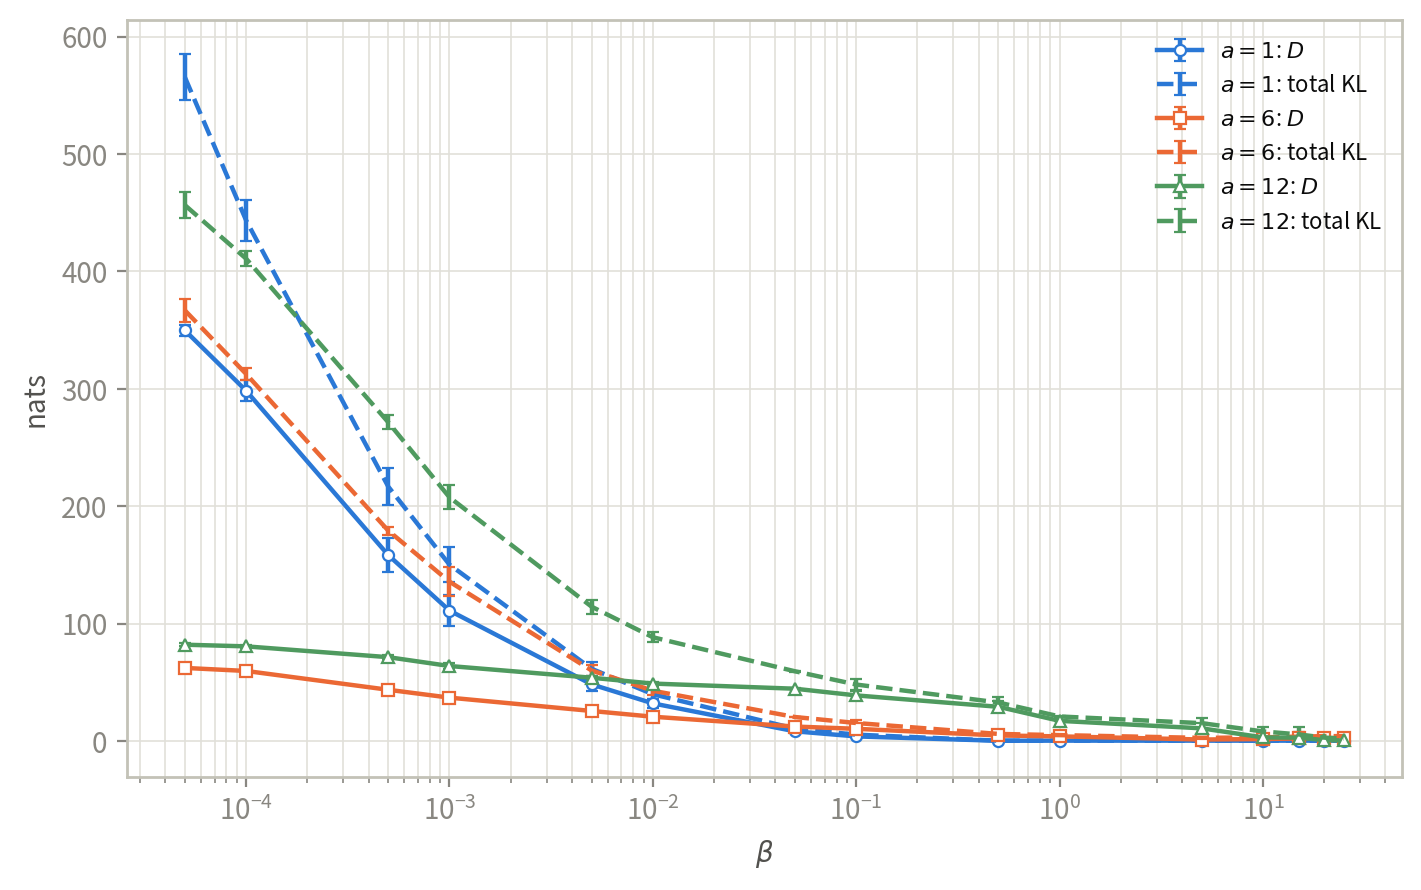
\includegraphics[width=0.48\linewidth]{figures/fig_mismatch_a_imagenet100_d_beta.png}\hfill
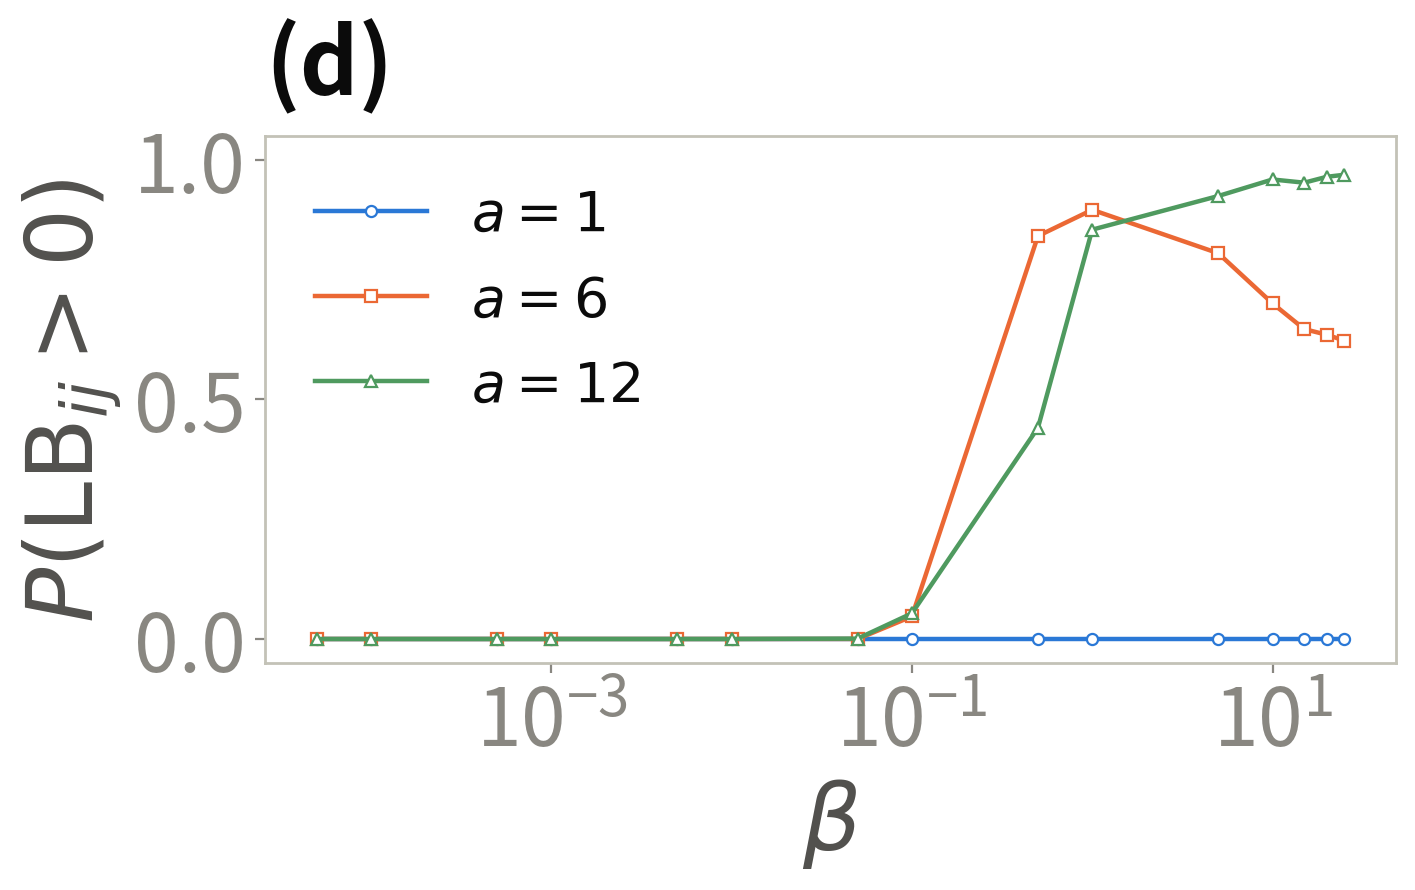
\includegraphics[width=0.48\linewidth]{figures/fig_mismatch_appendix_cls_ii_positive_fraction.png}
\caption{Alignment and separation diagnostics over the ImageNet-100 compression sweep. (a)
Anchor mismatch $\widehat D$ (solid) and total KL (dashed) against $\beta$, by
anchor scale. (b) Fraction of class pairs with a positive separation lower bound.}
\label{fig:direct-mismatch}
\end{minipage}\hfill
\begin{minipage}[t]{0.49\linewidth}
\centering
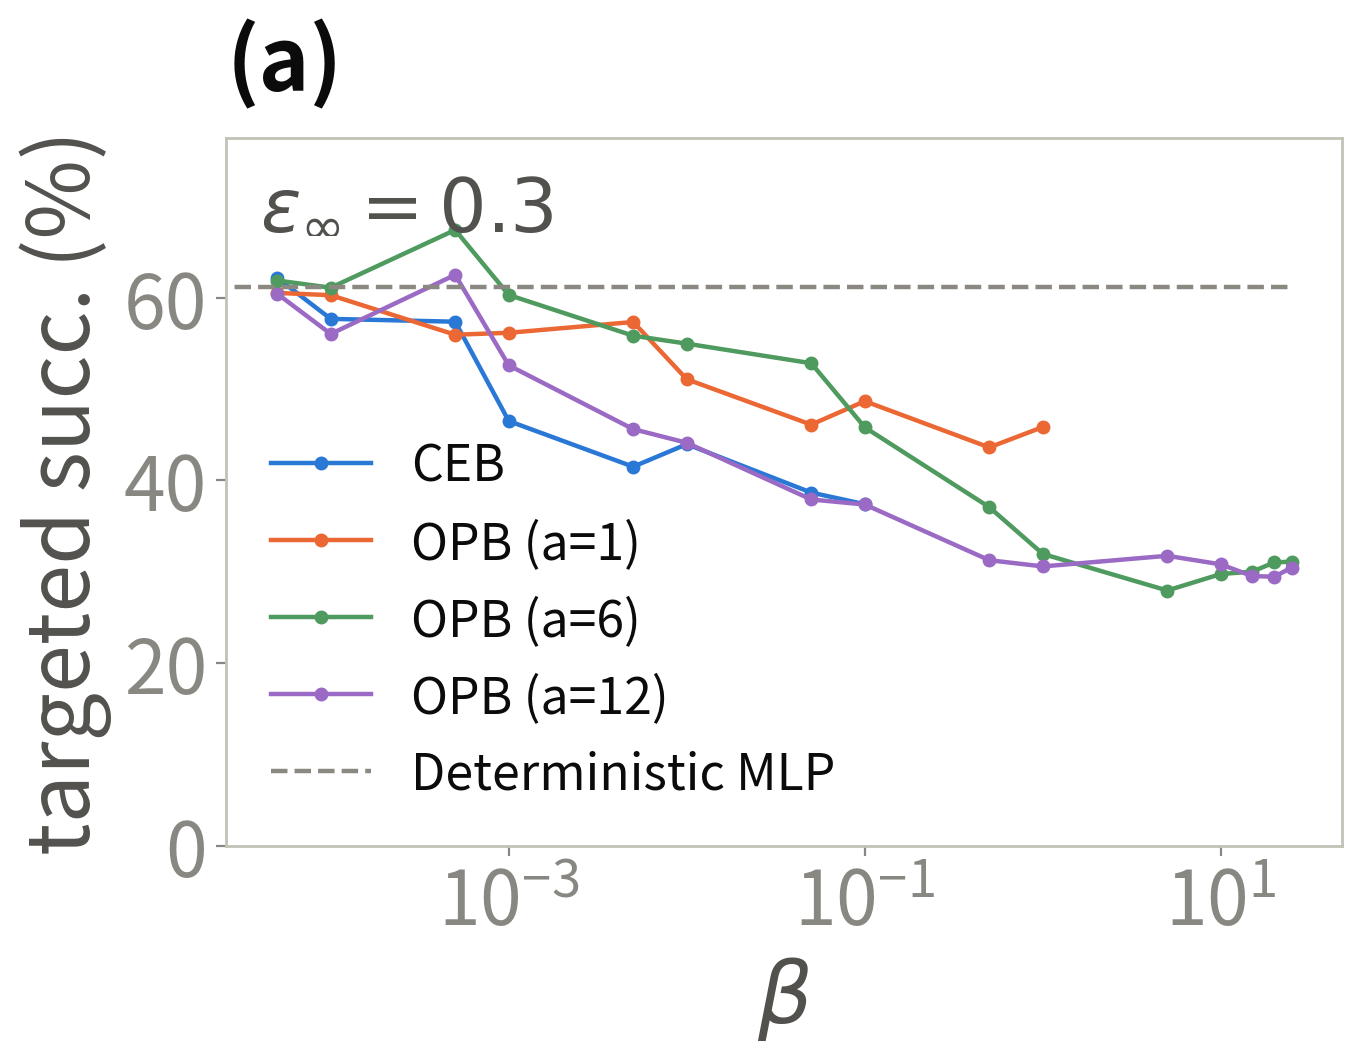
\includegraphics[width=0.48\linewidth]{figures/fig_adv_targeted_linf_mnist.png}\hfill
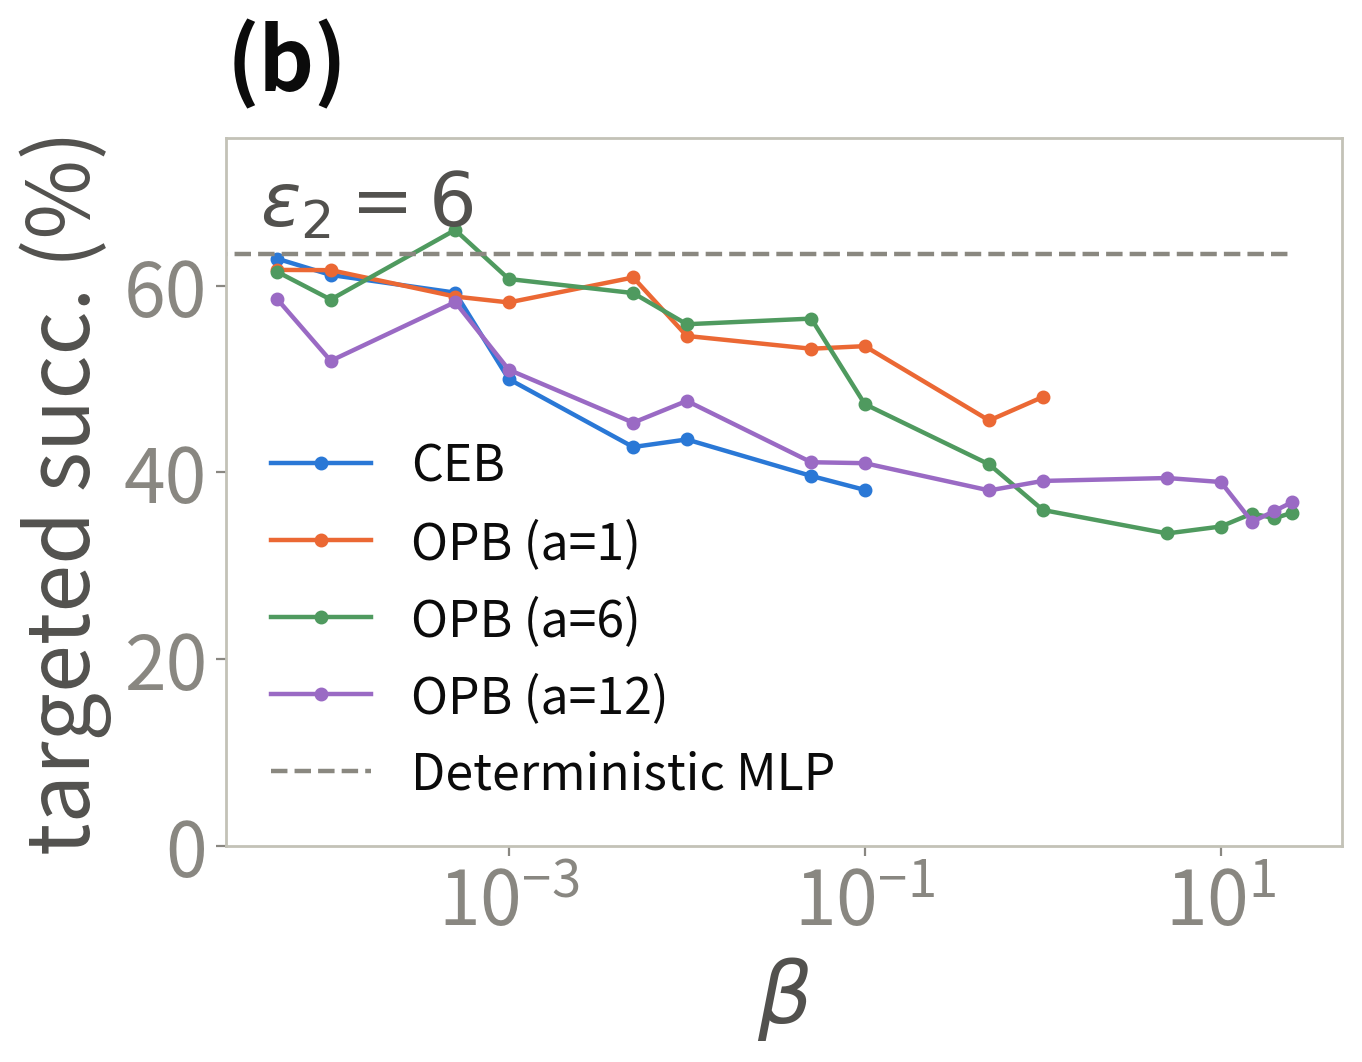
\includegraphics[width=0.48\linewidth]{figures/fig_adv_targeted_l2_mnist.png}
\caption{Targeted white-box PGD on MNIST (MLP): targeted success rate against $\beta$ under
(a) $L_\infty$, $\varepsilon=0.3$ and (b) $L_2$, $\varepsilon=6$. Curves are shown
only where stochastic clean accuracy exceeds $90\%$.}
\label{fig:robustness-main}
\end{minipage}
\end{figure*}


\subsection{Adversarial robustness}
\label{sec:robustness}
We use the targeted MNIST PGD protocol of CEB with EOT-10 gradients and 10-sample
stochastic predictions; each curve is shown only where the stochastic clean accuracy
exceeds $90\%$ (Fig.~\ref{fig:robustness-main}). Within that valid range, targeted
success falls monotonically with compression: every curve starts at the deterministic
baseline's level ($\approx61\%$ under $L_\infty$, $\approx63\%$ under $L_2$) and
declines by roughly a third to a half by the end of its valid range. The models
differ in how far that range extends. CEB's curve ends at $\beta=0.1$, where its
success ($37.4\%$/$38.1\%$) is matched by OPB $a=12$ ($37.4\%$/$41.0\%$); beyond it
CEB collapses toward chance accuracy, where near-zero success is trivial rather than
a robustness gain, so no later point is plotted. OPB $a=1$'s curve ends at
$\beta=1$, where its clean sampled-path accuracy drops below the $90\%$ validity
threshold. OPB $a=6,12$ stay valid over the
whole grid and continue to fall, reaching $31.1\%$/$30.5\%$ under $L_\infty$ and
$35.7\%$/$36.8\%$ under $L_2$ at $\beta=25$, roughly 30 points below the
deterministic baseline under $L_\infty$ and about 27 under $L_2$, with clean accuracy
still $\approx98\%$; the curves plateau from $\beta\ge5$ onward, so the gain sits in
the compressed operating point rather than in $\beta$ alone. Transfer attacks are reserved for the gradient-masking
check in Appendix~\ref{app:robustness}.


\subsection{Factor-wise ablations}
\label{sec:ablation}
The main comparison changes several factors simultaneously, so we also report a
paired intervention ladder that switches five design factors independently, namely
the prior geometry, the anchor scale, the readout, the IB term itself, and the
trainability of the prior frame, plus two
auxiliary contrasts on the prototype readout itself. Every
variant is trained on the three mechanism settings (MNIST, ImageNet-100, and
Cal.~Housing, all with MLP backbones) at its best
validation-selected configuration, and all comparisons are paired by seed. Each row
of Table~\ref{tab:ablation-ci} pairs two variants that differ in the factor named in
its first column; the variant definitions and the complete means are in
Appendix~\ref{app:ablation}.

\begin{table}[t]
\centering
\small
\setlength{\tabcolsep}{3pt}
\caption{Factor-wise paired differences (accuracy points on MNIST and
ImageNet-100; $95\%$ bootstrap percentile CIs; positive values favor the
first term).}
\label{tab:ablation-ci}
\begin{tabular}{l l c c}
\hline
factor & comparison & MNIST & ImageNet-100 \\
\hline
readout & GPB $-$ GPB-L & $+0.02$ [$_{-0.05}$, $_{0.08}$] & $+0.82$ [$_{0.34}$, $_{1.17}$] \\
readout (free geometry) & CEB-energy $-$ CEB & $-0.21$ [$_{-0.30}$, $_{-0.12}$] & $-1.19$ [$_{-1.50}$, $_{-0.96}$] \\
geometry & GPB $-$ CEB-energy & $+0.23$ [$_{0.10}$, $_{0.36}$] & $+2.63$ [$_{2.41}$, $_{2.88}$] \\
frame trainability & GPB $-$ OPB-RV & $+0.10$ [$_{0.05}$, $_{0.15}$] & $+0.83$ [$_{0.29}$, $_{1.19}$] \\
IB increment & GPB $-$ NCM-ortho & $+0.34$ [$_{0.22}$, $_{0.45}$] & $+1.89$ [$_{1.41}$, $_{2.36}$] \\
prototype structure & NCM-ortho $-$ NCM-learn & $-0.06$ [$_{-0.20}$, $_{0.11}$] & $+0.16$ [$_{-0.49}$, $_{0.82}$] \\
prototype readout alone & NCM-learn $-$ Base & $-0.16$ [$_{-0.28}$, $_{-0.05}$] & $-0.96$ [$_{-1.30}$, $_{-0.69}$] \\
\hline
\end{tabular}
\end{table}


The paired contrasts
(Table~\ref{tab:ablation-ci}; accuracy-point differences) rank
the factors on ImageNet-100: geometry is the largest ($+2.67$,
OPB-FS over CEB-energy), followed by the IB term ($+1.89$, GPB over NCM-ortho, which
additionally contains frame trainability) and the tied readout ($+0.82$, GPB over
GPB-L), while fixing the anchor scale costs essentially nothing ($-0.04$, GPB over
OPB-FS). Two patterns matter as much as the ranking. First, the readout contrast
flips sign with the accompanying geometry: on the free-geometry side the energy
readout costs $1.19$ points (CEB-energy below CEB), so restricting the readout helps
only when the geometry it ties to is the constructed one. Second, the prototype machinery contributes nothing on its own: NCM-learn trails
the plain backbone by $0.96$ points, and fixing its prototypes to the orthogonal
frame without the IB term is a null ($+0.16$, CI spanning zero), so neither the
energy form nor the frozen geometry is the source of the gain. On MNIST all contrasts
shrink to within $0.35$ points, so the ladder
resolves factors only where the task margin is large enough. The frozen-prior
ablation (Appendix~\ref{app:ablation}) shows the trainable frame carries task
benefit on classification: GPB exceeds the variant with all prior parameters
frozen by $+0.10$ on MNIST and $+0.83$ on ImageNet-100
(Table~\ref{tab:ablation-ci}, frame trainability). These interventions
change the fitted training problem and therefore support factor-wise attribution,
not a unique causal decomposition.

\subsection{Compression sweeps}
\label{sec:sweep}
This subsection shows the classification sweep on ImageNet-100 (MLP):
test accuracy and realized conditional KL against $\beta$, for CEB and OPB at anchor
scales $a\in\{1,6,12\}$ (Fig.~\ref{fig:compression-main}a,b); the California Housing
regression companion is in Appendix~\ref{app:compression}.

\begin{figure*}[t]
\centering
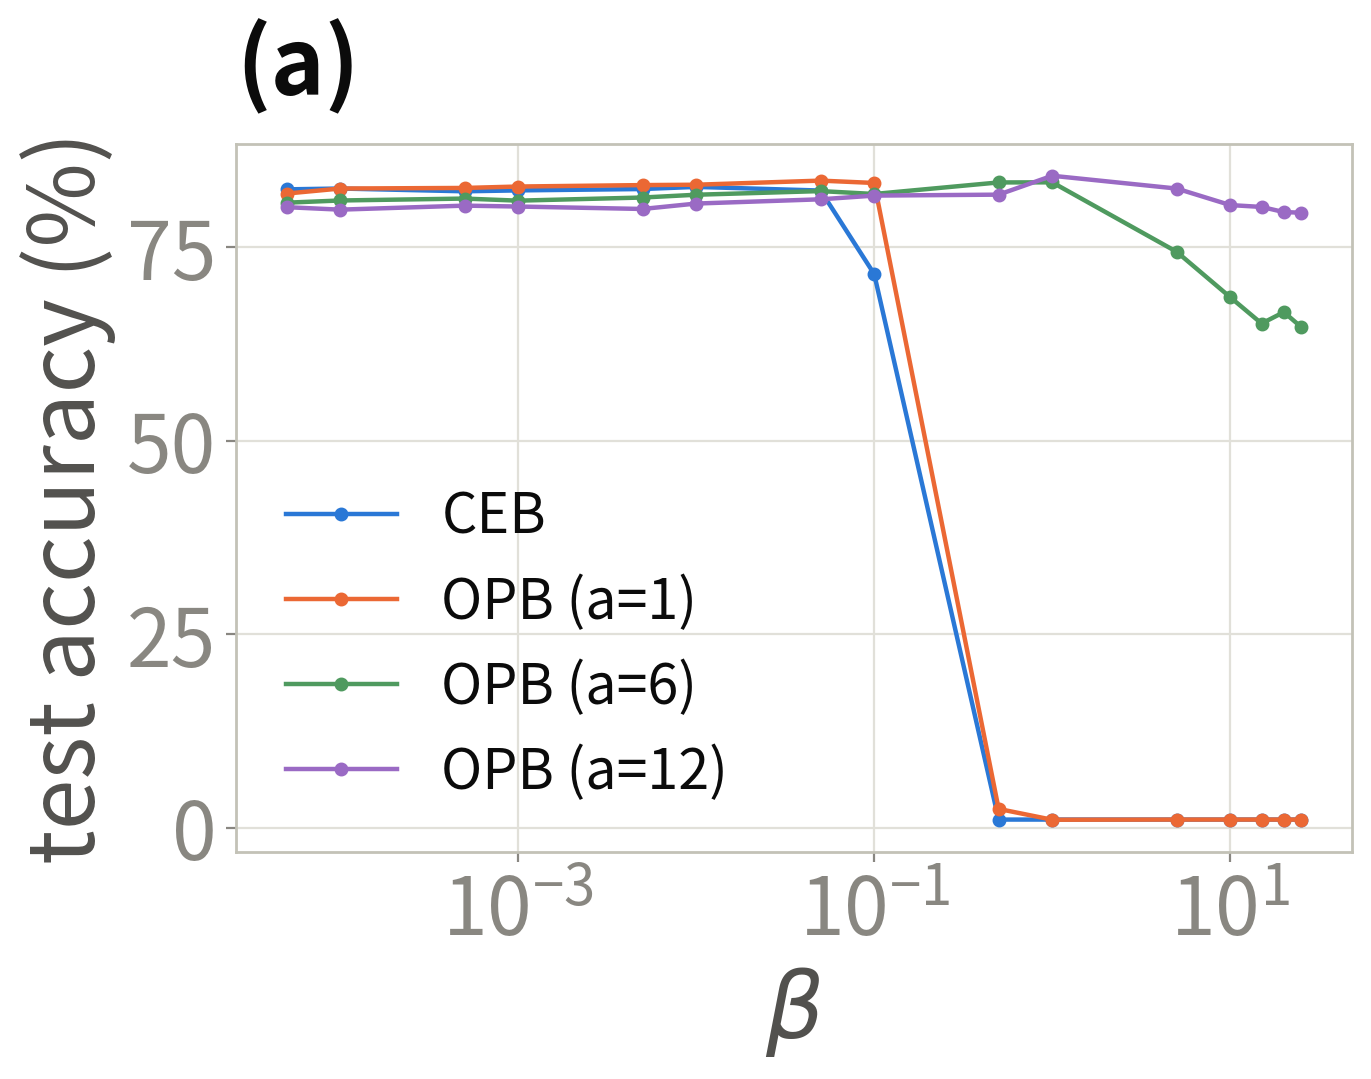
\includegraphics[width=0.24\linewidth]{figures/fig_beta_acc_imagenet100.png}\hfill
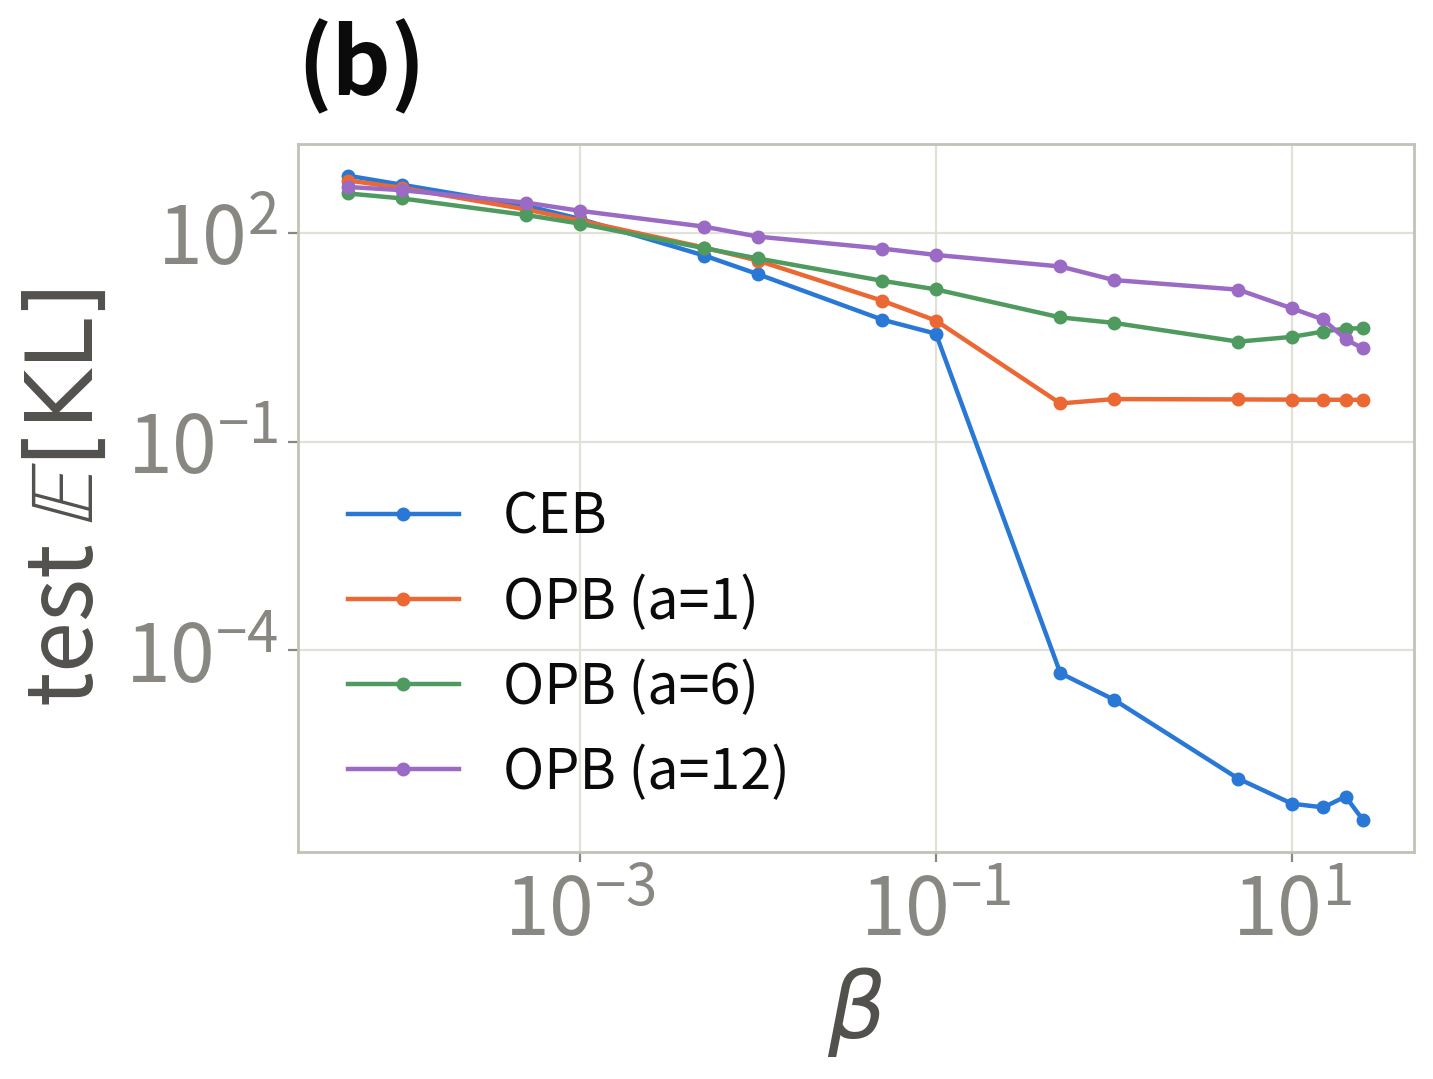
\includegraphics[width=0.24\linewidth]{figures/fig_beta_kl_imagenet100.png}\hfill
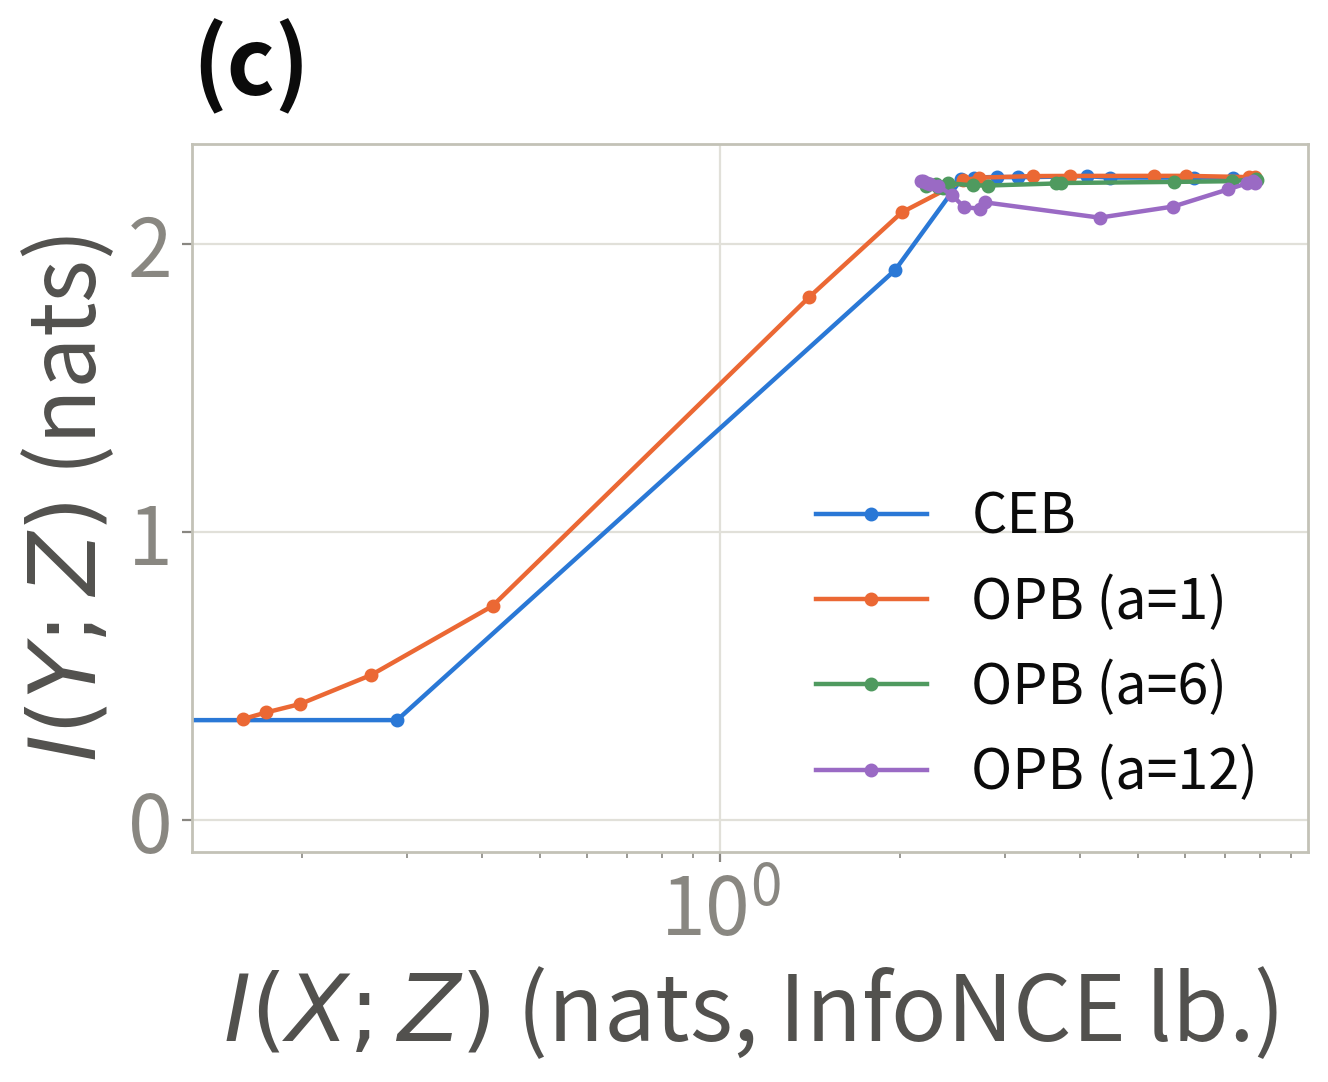
\includegraphics[width=0.24\linewidth]{figures/fig_info_plane_mnist.png}\hfill
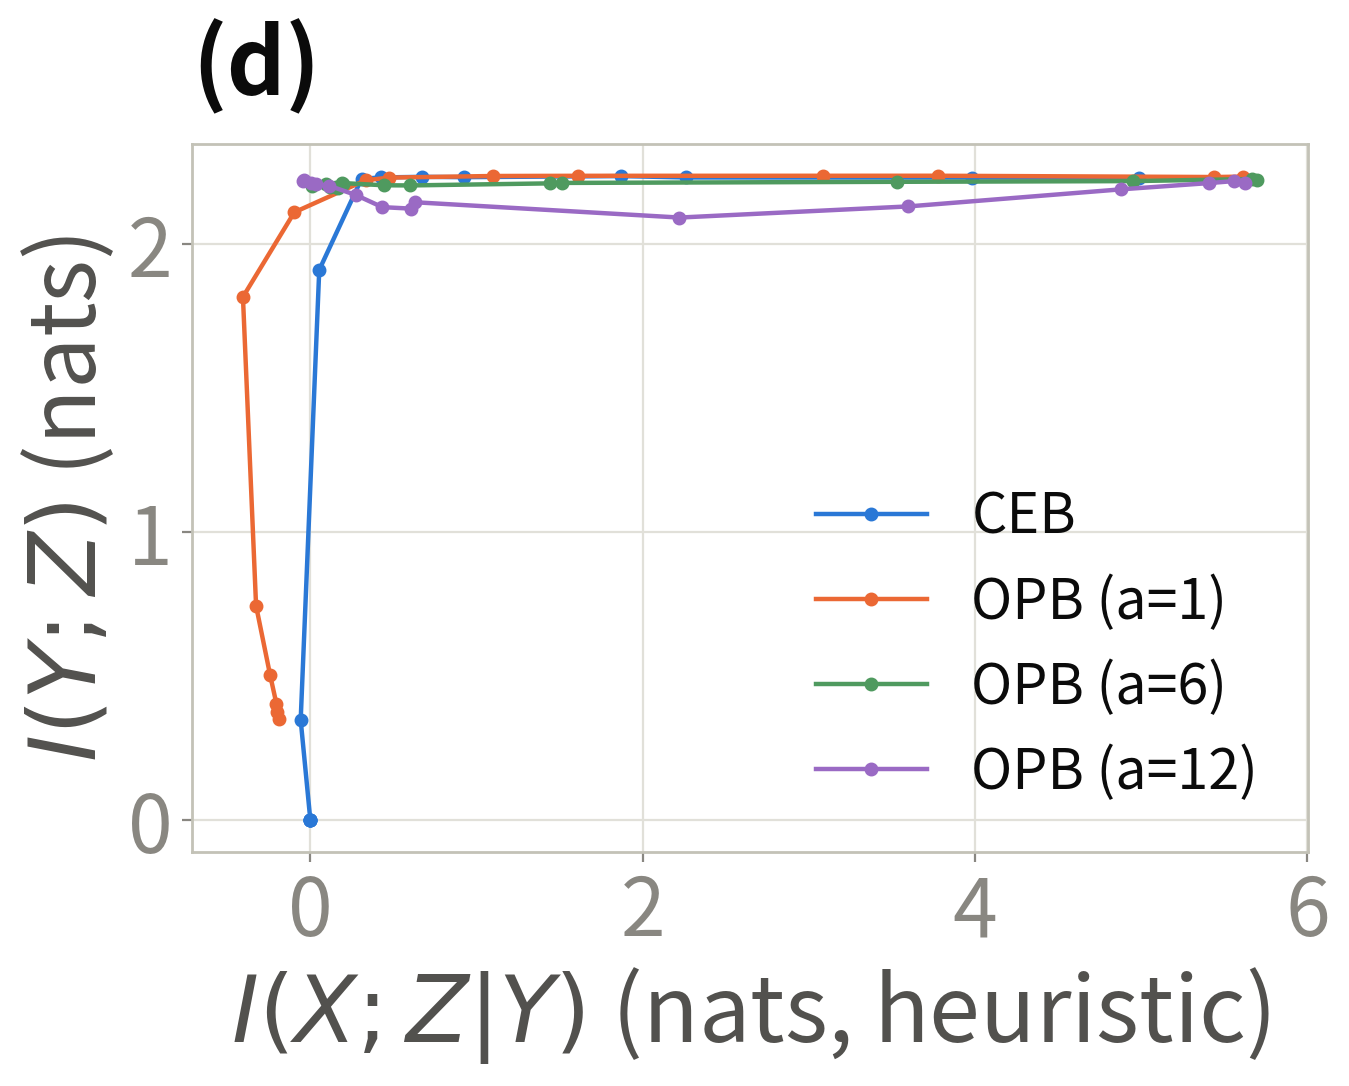
\includegraphics[width=0.24\linewidth]{figures/fig_certificate_plane_mnist.png}
\caption{Compression behavior across two views and two tasks. (a)--(b)
ImageNet-100 classification sweep (MLP): test accuracy and realized conditional KL
against $\beta$. (c)--(d) MNIST information-plane and
certificate-plane estimates.}
\label{fig:compression-main}
\end{figure*}

Larger anchor scales retain the high-accuracy plateau farther into strong
compression: $a=12$ keeps $79.4\%$ accuracy at $\beta=25$, where CEB has already
left its valid high-accuracy range and $a=1$ collapses, while at weak compression
larger scales pay a one-to-three point cost. The trade-off reverses under stronger
compression, where the $a=12$ scale is the most accurate configuration on the grid
($\beta\ge1$). The KL panel shows where the two
objectives spend the penalty: CEB's KL falls from $3.6$ at $\beta=0.1$ to
$\sim10^{-5}$ at $\beta=0.5$ because its learned reference shrinks to absorb the
term, whereas OPB's KL stays anchored at the geometric scale of its fixed prior
($48$ at $\beta=0.1$, $21$ at $\beta=1$) and is dominated by anchor alignment, so
the structure is retained rather than absorbed. Together the curves make the
anchor-scale/compression trade-off visible across the useful operating range.
The complementary scale-axis view, reading the full nine-point scale
grid at three fixed $\beta$ levels, is reported in
Appendix~\ref{app:scale-sensitivity}.

\subsection{Information-plane diagnostic}
\label{sec:info-plane}
The MNIST information-plane estimates provide a second view of the compression
behavior (Fig.~\ref{fig:compression-main}c,d). They are estimator-level diagnostics;
the matched table and estimator details
are in Appendix~\ref{app:info-plane}, with the Housing companion in
Appendix~\ref{app:info-plane-extra}.

The two planes show what each method discards as compression deepens. In the
information plane (Fig.~\ref{fig:compression-main}c, log $I(X;Z)$ axis), CEB follows
the classic corner: compression and task information fall together, from
$I(X;Z)=2.54$ nat at $\beta=0.1$ to $1.96$ nat at $\beta=0.5$, and by $\beta=1$
both are near zero. OPB with $a=6,12$ compresses from $\approx7.9$ to $\approx2.2$
nat but never below it, with $I(Y;Z)$ flat just below the $H(Y)=\ln10$ ceiling, so
compression stops at the task-information level, consistent with the aligned-model
Fano lower bound of Corollary~\ref{cor:opb-fano}. OPB with $a=1$ tracks $a=6,12$ until
$\beta=0.5$ and then collapses toward CEB's corner, with $I(Y;Z)$ falling to
$0.17$--$0.45$ nat. The certificate plane
(Fig.~\ref{fig:compression-main}d) reads the same contrast as where each trajectory
ends: CEB and OPB with $a=1$ reach zero residual together with the
task-information collapse, whereas $a=6,12$ terminate at full task height on a
stable nonzero residual plateau of $0.20$--$0.46$ nat.

\subsection{Geometry transfer}
\label{sec:mechanism}
At matched compression $(\beta,a,\rho)=(0.1,12,12)$, the posterior geometry is read
directly off the class-center cosine Gram matrices (Fig.~\ref{fig:mechanism-main}a,b;
Table~\ref{tab:mechanism-main}): OPB's Gram is visually an identity matrix, whereas
CEB's shows visible off-diagonal structure with no clean pattern. The posterior thus
inherits the constructed orthogonal frame, which is exactly what the zero-parameter
tied readout relies on. On Housing (Fig.~\ref{fig:mechanism-main}c,d), the axial
scatter shows the same contrast: EPB's points hug its prior line, whereas CEB's cloud
deviates from its prior line's direction and its learned axis scale swings across
runs: its geometry is neither aligned with its reference nor stable across runs. The
tied-metric column of Table~\ref{tab:mechanism-main} shows the payoff: the tied heads
attain $98.44\%$ on MNIST against CEB's $98.16\%$, and $R^2=0.778$ on Housing against
$0.491$.

\begin{figure*}[t]
\centering
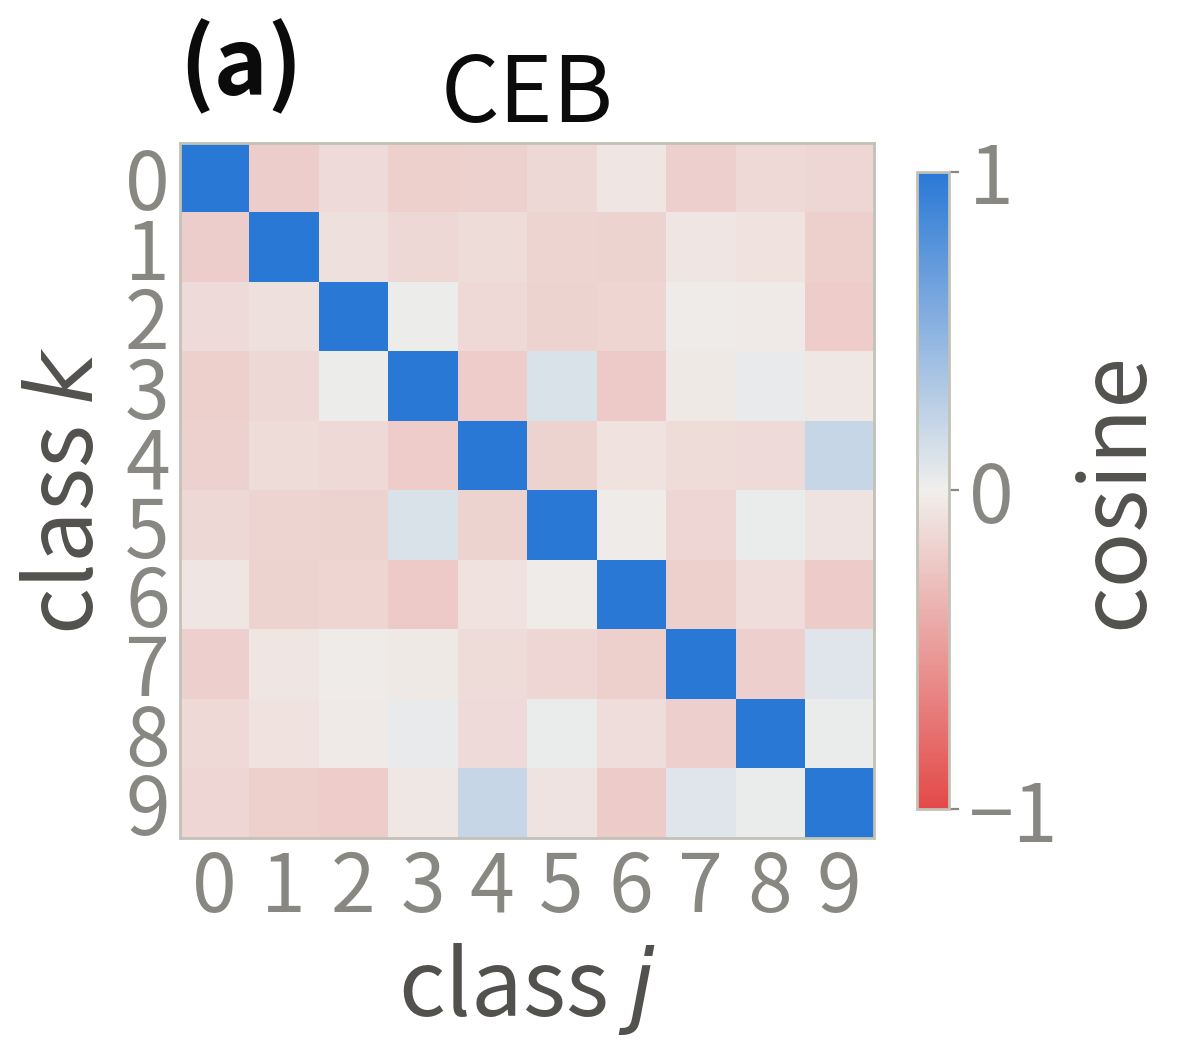
\includegraphics[width=0.24\linewidth]{figures/fig_mechanism_gram_ceb.png}\hfill
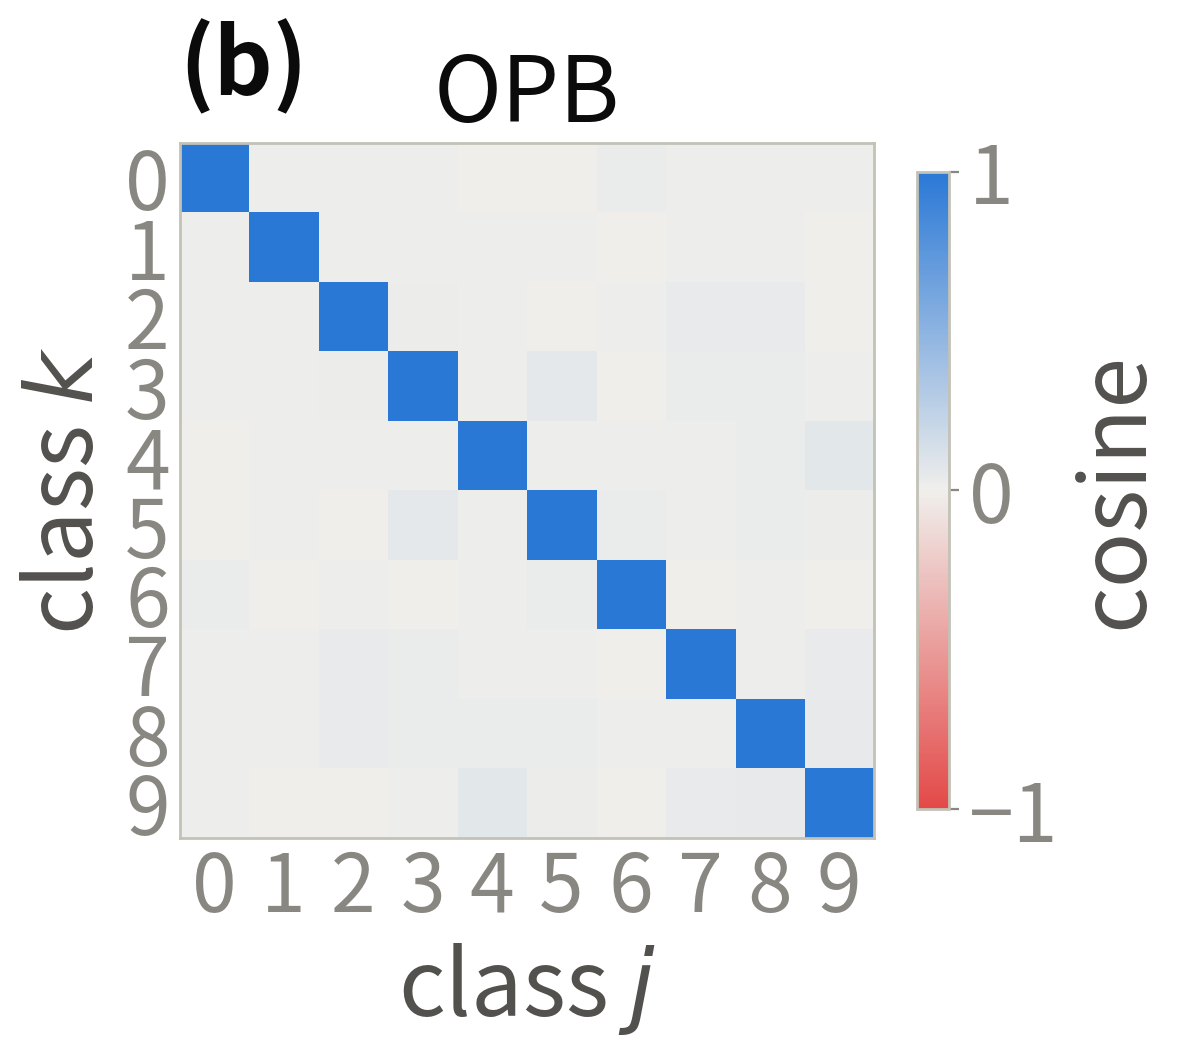
\includegraphics[width=0.24\linewidth]{figures/fig_mechanism_gram_opb.png}\hfill
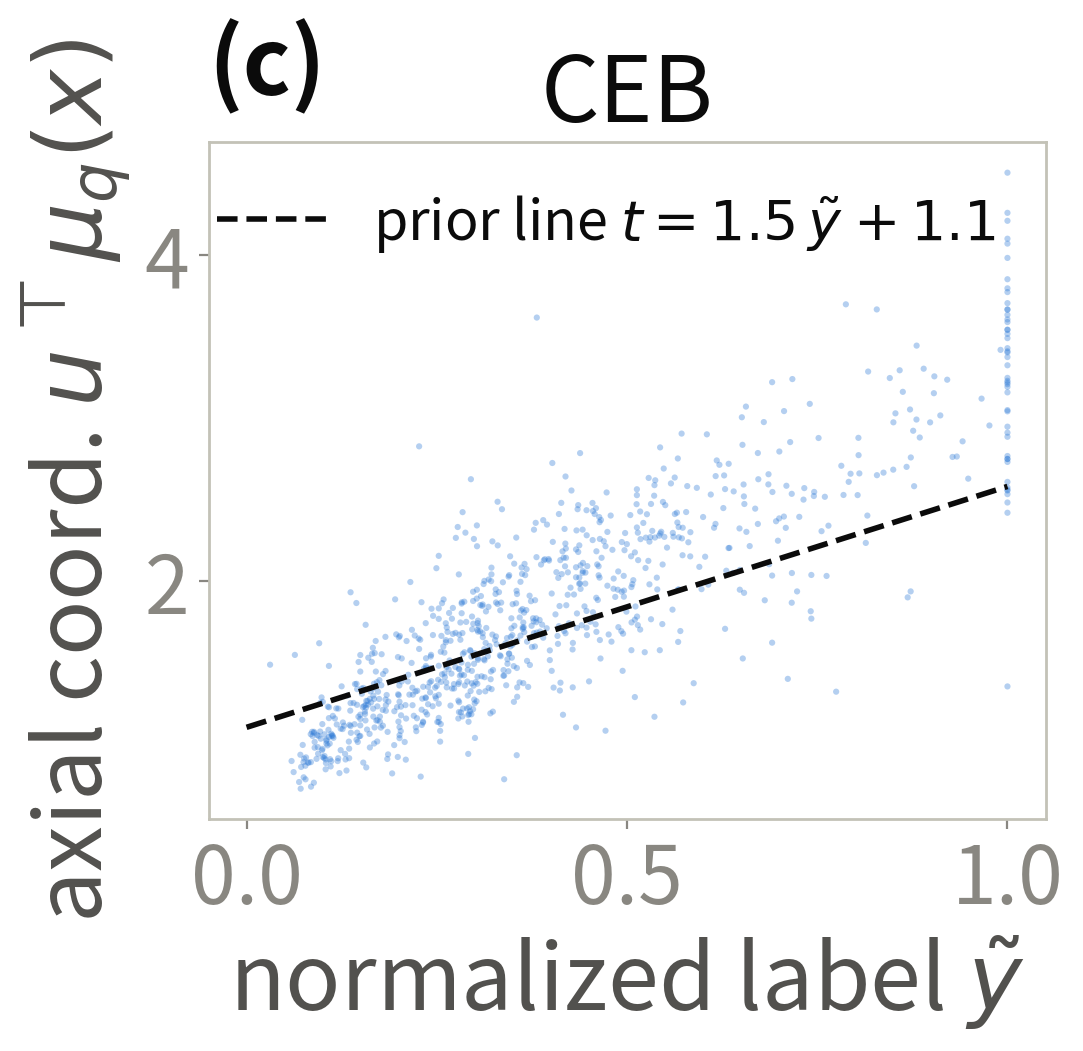
\includegraphics[width=0.24\linewidth]{figures/fig_mechanism_axis_ceb.png}\hfill
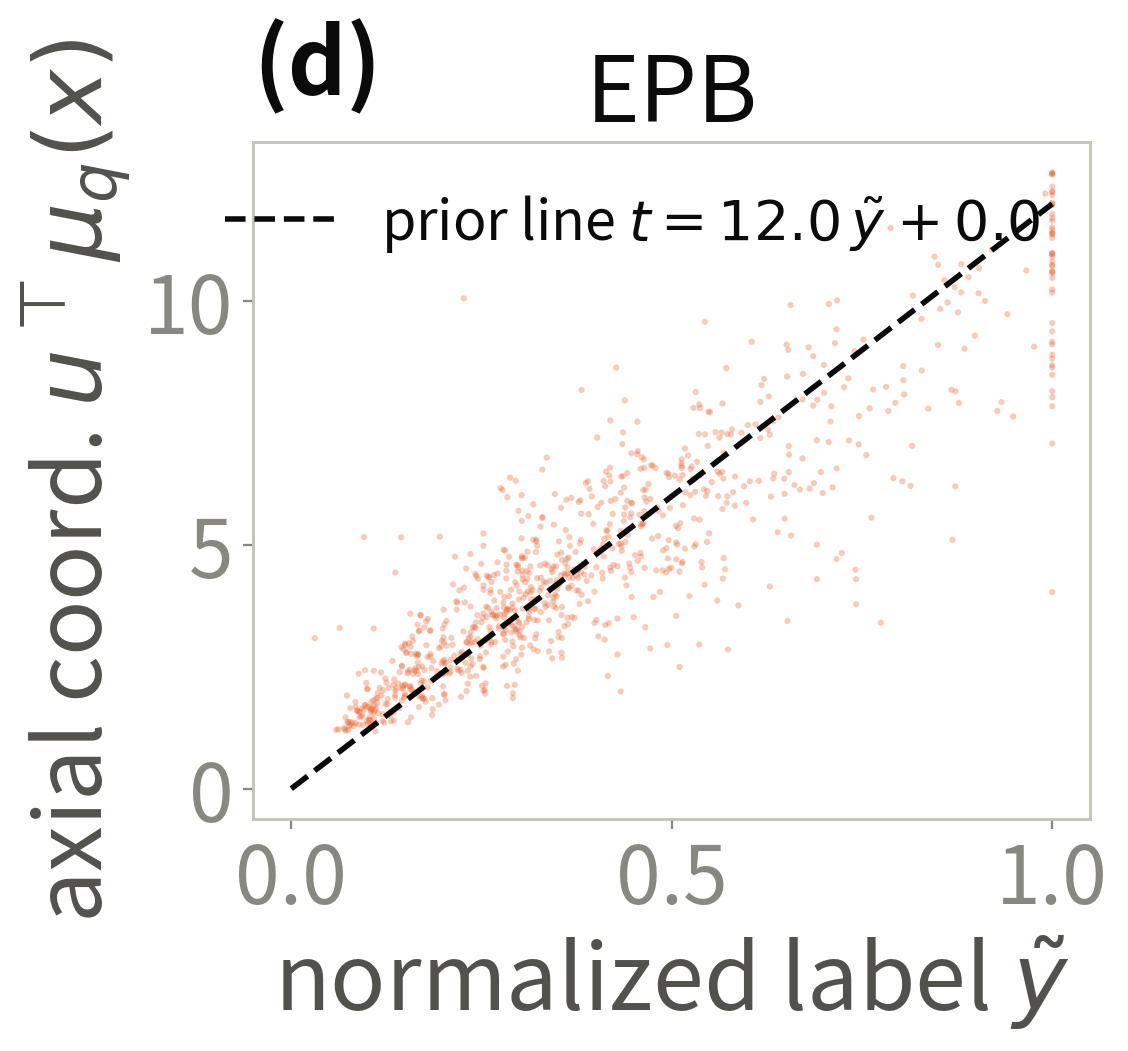
\includegraphics[width=0.24\linewidth]{figures/fig_mechanism_axis_epb.png}
\caption{Posterior geometry: class-center Gram
matrices for (a) CEB and (b) OPB, and axial coordinates for (c) CEB and (d) EPB.}
\label{fig:mechanism-main}
\end{figure*}

\begin{table}[t]
\centering\small
\setlength{\tabcolsep}{3pt}
\caption{Posterior-geometry statistics: geometry concentration (mean absolute
off-diagonal cosine of the class-center Gram; off-axis fraction for Housing), scale
following (posterior center norm against the declared anchor scale; slope against
$\rho$ for Housing), tied metric (accuracy or $R^2$ under the tied head), and
cross-seed stability (standard deviation of the concentration across runs).}
\label{tab:mechanism-main}
\begin{tabular}{l c c c c}
\hline
Model & Geometry concentration & Scale following & Tied metric & Cross-seed stability \\
\hline
CEB (MNIST) & $0.1205\pm0.0026$ & $5.14$ & $98.16\%$ & $0.0201$ \\
OPB (MNIST) & $0.0203\pm0.0021$ & $11.00$ & $98.44\%$ & $0.0082$ \\
CEB (Housing) & $0.0233$ & $2.65\pm0.59$ & $R^2=0.491$ & $0.593$ \\
EPB (Housing) & $0.0002$ & $9.22\pm0.15$ & $R^2=0.778$ & $0.155$ \\
\hline
\end{tabular}
\end{table}

\paragraph{Conclusion and limitations.} The experiments form a consistent
progression from construction to behavior: the baseline table establishes end-to-end
utility across modalities; the factor interventions attribute the gain to the
geometric prior; the controlled noise study matches the analytic ambiguity floor; and
the mismatch, robustness, compression, information-plane, and geometry diagnostics
show how the declared prior is reflected in the learned posterior at different
operating points. Constraining the conditional prior changes the geometry available
to the KL, and the tied readout makes that geometry visible to prediction; the
measured mismatch determines how much of the declared geometry transfers.

The results are qualified accordingly. The mismatch bound is comparator-relative: on
a real benchmark its floor is determined by a prespecified comparator and its label,
mean-approximation, and covariance terms rather than an intrinsic dataset constant,
and the separation lower bound is informative only when the realized mismatch stays
below the declared margin. The orthogonal frame fixes all pairwise anchor
distances, so the framework does not claim to recover arbitrary semantic class
similarities; the trainable frame is a rotation channel whose certificate-zero set
contains full-retention rotated codes, so the framework pins the geometry of the
code rather than the retained label information. Data-driven comparator certificates
and tighter information estimates are natural
next steps. Proofs and all
supplementary evidence are collected in Appendices~\ref{app:theory}--\ref{sec:related}.
